\subsection{Branches and Tags}

Technically Subversion does not introduce separate concepts for branches and tags. Both branches and tags are versioned directories under repository root. As result Translator performs theirs translation in similar way. There are differences at Git level only:
\begin{enumerate}
	\compactlist
	\item Addition.
	\begin{itemize}
		\item Creation of /branches/\emph{B} directory leads to creation of a new branch reference \emph{B}.
		\item Creation of /tags/\emph{T} directory leads to addition of corresponding Tag Object with name \emph{T}.
	\end{itemize}
	\item Modification.
	\begin{itemize}
		\item Change at /branches/\emph{B} directory leads to updating of corresponding branch reference \emph{B}.
		\item Change at /tags/\emph{T} directory leads to the removal of obsolete Tag Object with name \emph{T} and creation of new Tag Object with the same name for corresponding Commit Object.
	\end{itemize}
	\item Deletion.
	\begin{itemize}
		\item Removal of /branches/\emph{B} directory leads to removal of corresponding reference \emph{B} at Git repository, when
		\item Removal of /tags/\emph{T} directory leads to removal of corresponding Tag Object with name \emph{T}.
	\end{itemize}
\end{enumerate}

The same rules could be treated in opposite direction --- every change of Git branch or tag leads to corresponding change of Subversion branch or tag.

This and further chapters consider scenarios with branches only. But every scenario could be applied to tags with the rules above taken into account.

\subsubsection{From Subversion to Git}

There is a number of ways to create branch in Subversion.

\begin{enumerate}
\compactlist
\item Branch creation by copying, figure \ref{branch_creation_svn_to_git}.

\begin{figure}[!h]
\centering
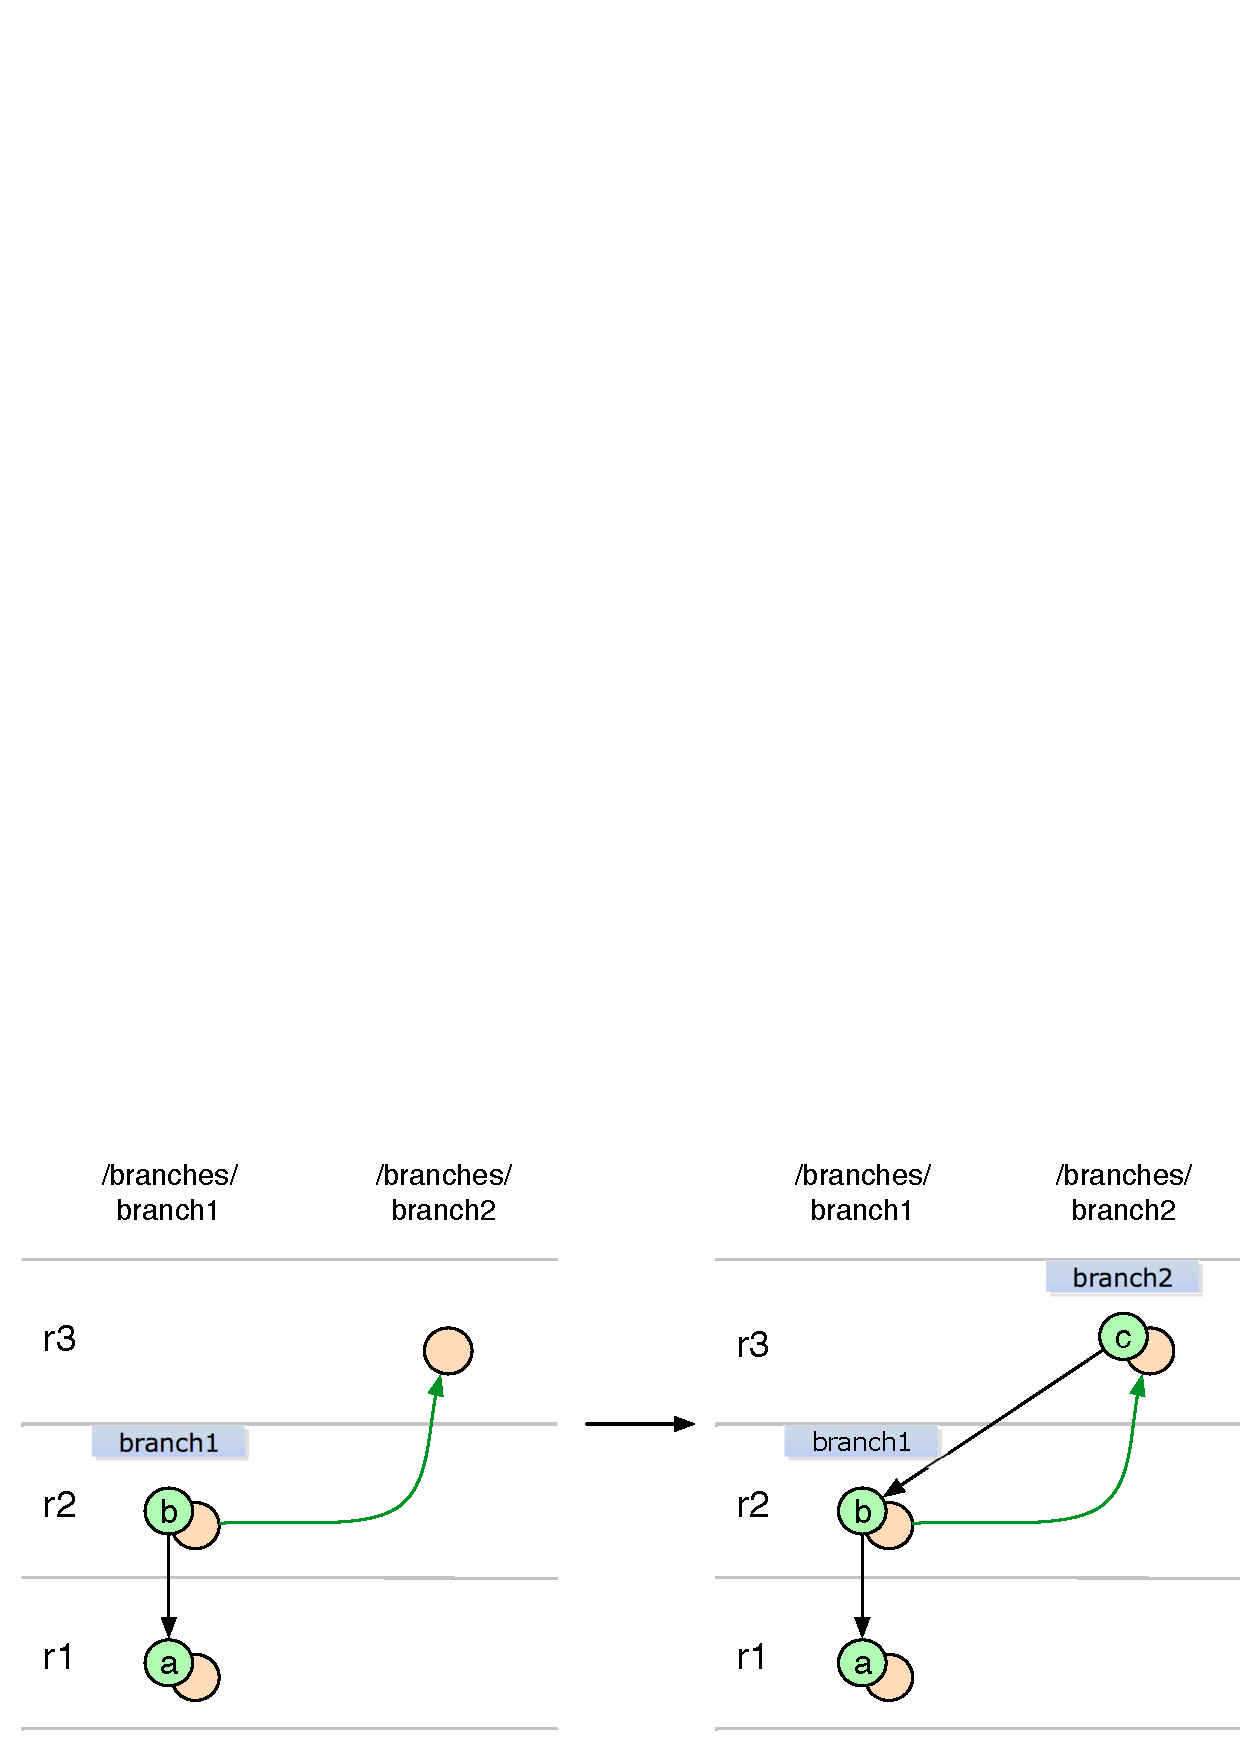
\includegraphics[width=\linewidth]{img/diagrams/branch_creation_svn_to_git.pdf}
\caption{Subversion branch copying being translated to Git branch creation.}
\label{branch_creation_svn_to_git}
\end{figure}

% end of item
\item Branch addition with merge history. See \ref{branch_creation_from_mergeinfo_svn_to_git}.

\begin{figure}[!h]
\centering
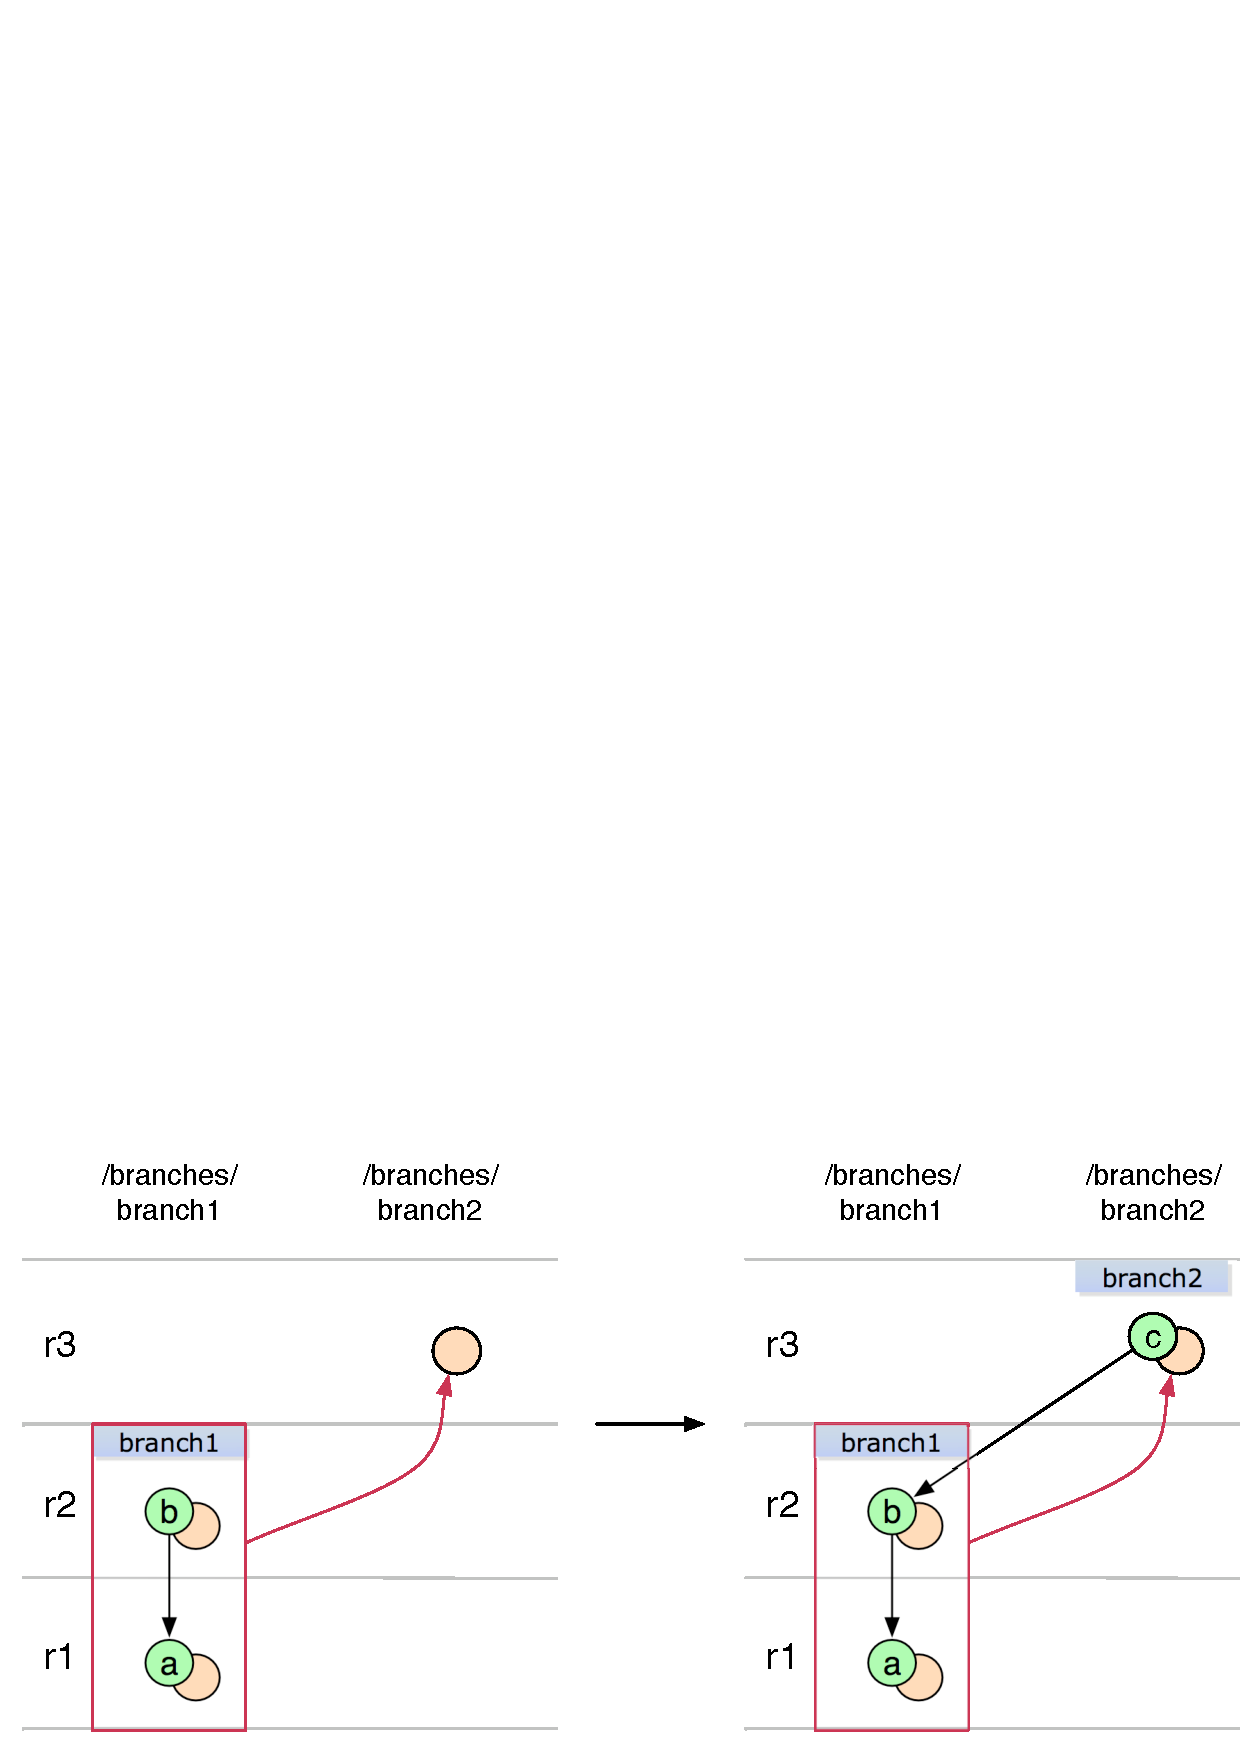
\includegraphics[width=\linewidth]{img/diagrams/branch_creation_from_mergeinfo_svn_to_git.pdf}
\caption{Subversion branch addition being translated to Git branch creation.}
\label{branch_creation_from_mergeinfo_svn_to_git}
\end{figure}

\item Branch addition with no history.

This kind of translation basically consists of:
\begin{enumerate}
	\item Creation of new commit object with no parents attached to it.
	\item Adding a branch reference to this new commit afterwards.
\end{enumerate}

\end{enumerate}

\subsubsection{From Git to Subversion}

\begin{enumerate}
\compactlist
\item Branch creation and committing on new branch, figure \ref{branch_creation_git_to_svn}.

\begin{figure}[!h]
\centering
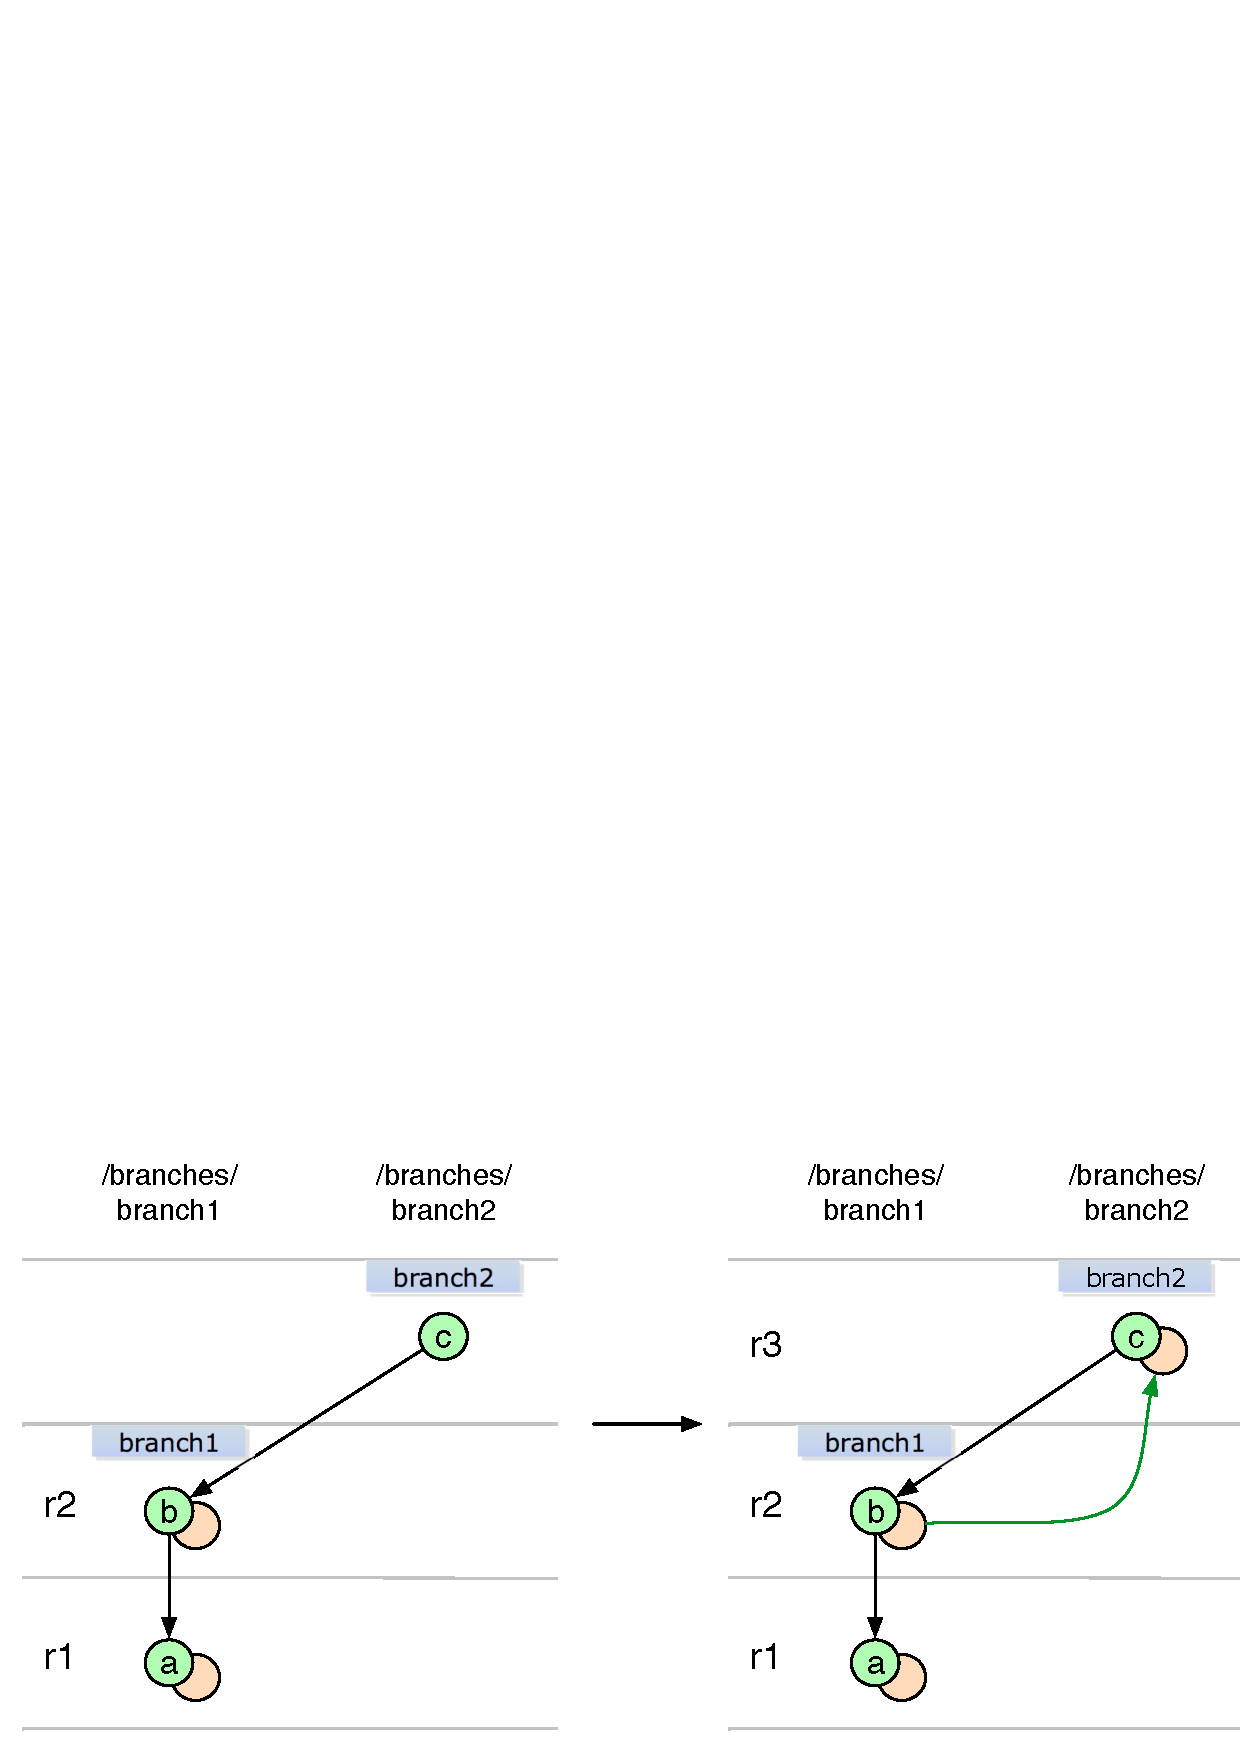
\includegraphics[width=\linewidth]{img/diagrams/branch_creation_git_to_svn.pdf}
\caption{Commit on Git branch being translated to Subversion.}
\label{branch_creation_git_to_svn}
\end{figure}

\item Branch reference creation with no commit, figure \ref{svn_no_change_branch_creation_git_to_svn}.

\begin{figure}[!h]
\centering
\includegraphics[width=\linewidth]{img/diagrams/svn_no_change_branch_creation_git_to_svn.pdf}
\caption{Commit on Git branch being translated to Subversion.}
\label{svn_no_change_branch_creation_git_to_svn}
\end{figure}

\item Double branch reference creation and committing on new branches, figure \ref{ambiguous_svn_branch_git_to_svn}.

\begin{figure}[!h]
\centering
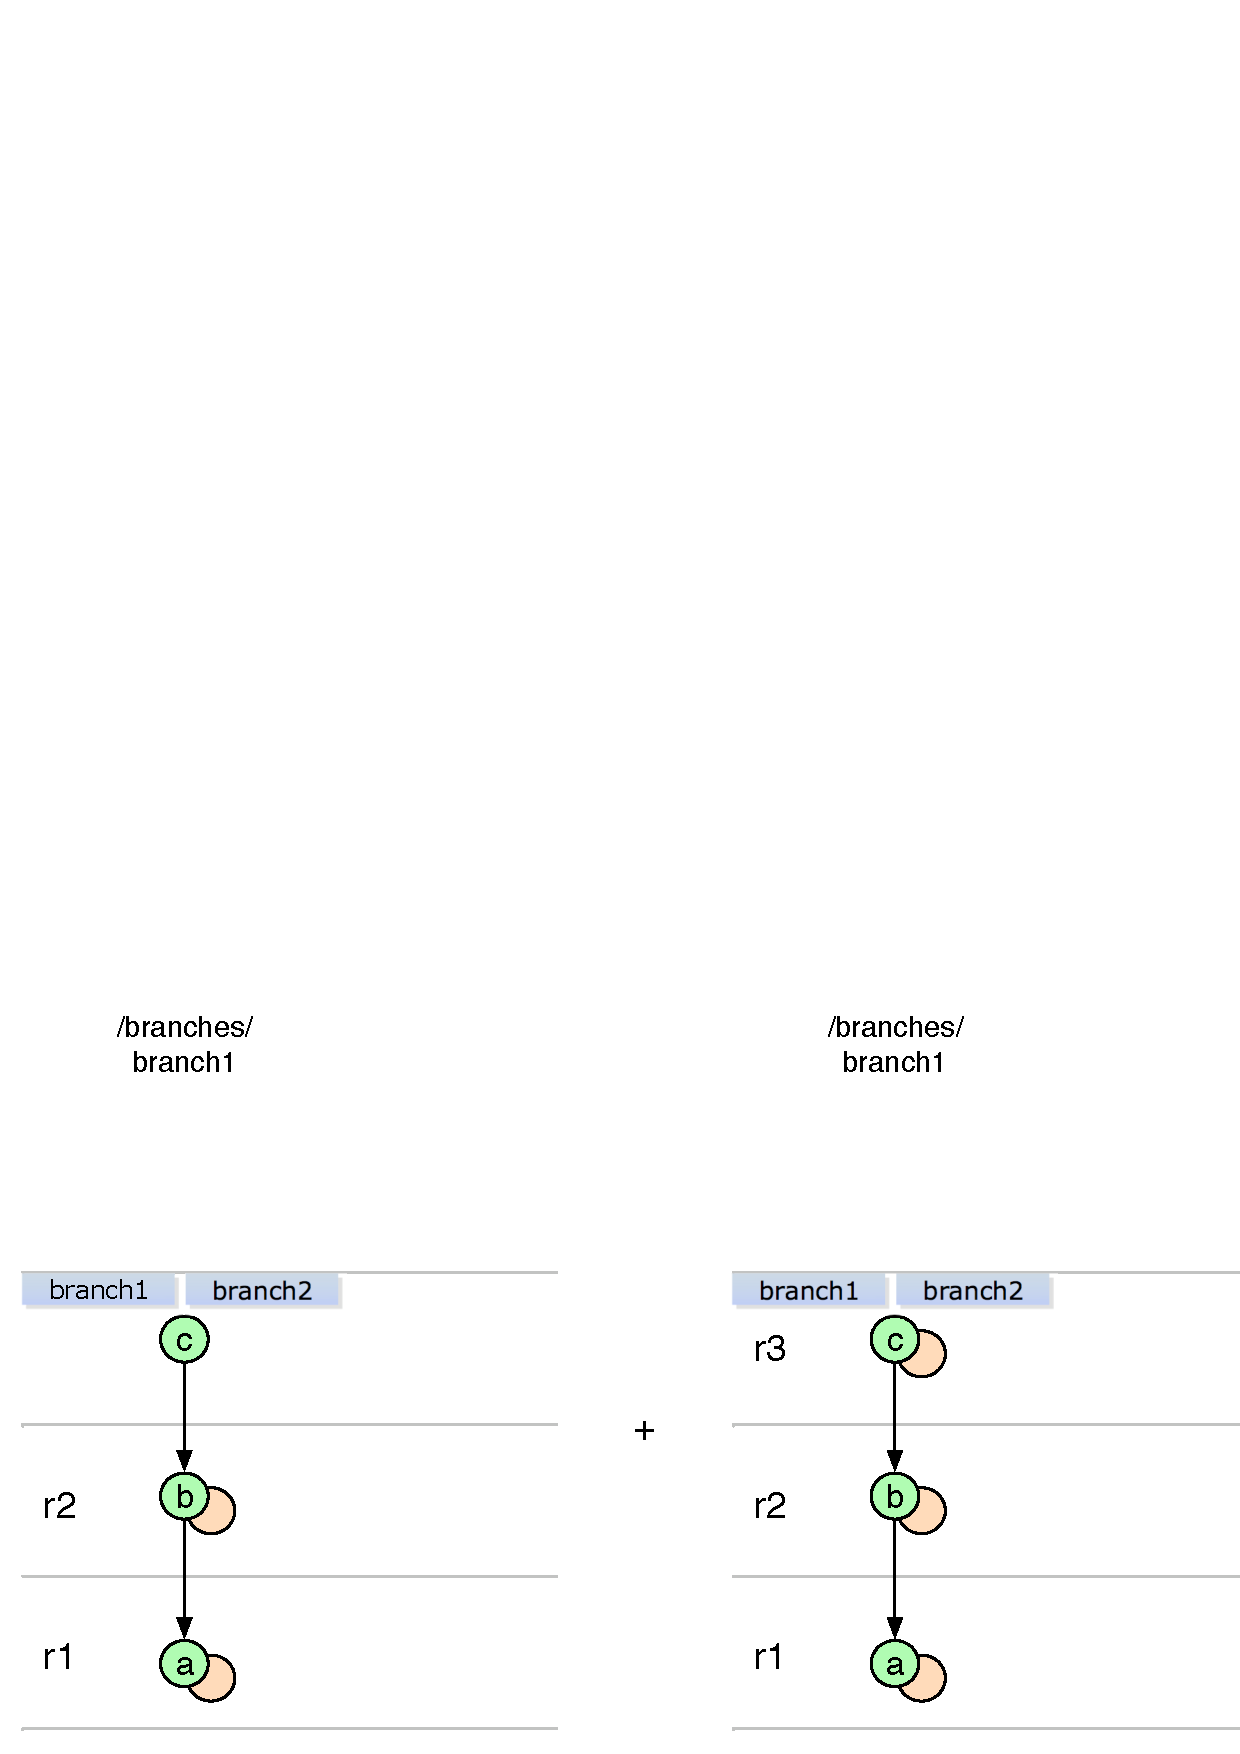
\includegraphics[width=\linewidth]{img/diagrams/ambiguous_svn_branch_git_to_svn.pdf}
\caption{Commit on Git branch being translated to Subversion.}
\label{ambiguous_svn_branch_git_to_svn}
\end{figure}

\end{enumerate}
